\documentclass[11pt]{article}
\usepackage[margin=0.92in]{geometry}
\usepackage{amsmath,amssymb,amsthm}
\usepackage{graphicx}
\usepackage{microtype}
\usepackage{xcolor}
\usepackage{enumitem}
\usepackage{placeins}
\usepackage[colorlinks=true,linkcolor=blue!55!black,citecolor=blue!55!black,urlcolor=blue!55!black]{hyperref}

\newtheorem{theorem}{Theorem}
\newtheorem{proposition}[theorem]{Proposition}
\newtheorem{lemma}[theorem]{Lemma}
\newtheorem{corollary}[theorem]{Corollary}
\newcommand{\R}{\mathbb R}
\newcommand{\C}{\mathbb C}
\newcommand{\F}{\mathcal F}

\title{Asymmetric weights break real-analytic functional calculus\\
\large A counterexample to Theorem 1.5 of arXiv:2507.16516 as printed}
\author{Automated Mathematics Run \texttt{fa\_banach\_001}, lane 10}
\date{9 August 2026}

\begin{document}
\maketitle

\begin{center}
\fcolorbox{blue!55!black}{blue!4}{\parbox{0.90\textwidth}{
\textbf{Status.} Candidate full counterexample, subject to human
verification.  For every fixed $1\le q<\infty$, there is an admissible
regular-growth weight $\omega$ on $\R$---also a $q$-algebra weight when
$q>1$---such that $A^q_\omega(\R)$ is not closed under complex
conjugation.  Thus the real-analytic map $F(z)=\overline z$, $F(0)=0$,
refutes Theorem 1.5 under the paper's explicit definition of a weight.
Moreover, closure under conjugation is characterized exactly by
$\omega(x)\asymp\omega(-x)$ almost everywhere.}}
\end{center}

\section{Source statement and the missing hypothesis}

The source is D.~G.~Bhimani and K.~B.~Solanki,
\emph{On the weighted Wiener--L\'evy theorem: analogue on Euclidean space,
strong converse on LCA group and applications to modulation
spaces}~\cite{BS}, arXiv:2507.16516v2.

For a locally compact abelian group $G$, the paper defines a weight to be a
measurable map $\omega:G\to[1,\infty)$ satisfying
\[
 \omega(x+y)\le \omega(x)\omega(y).
\]
It calls $\omega$ admissible when it satisfies the Beurling--Domar condition
\[
 \sum_{n\ge1}\frac{\log\omega(nx)}{n^2}<\infty
 \qquad(x\in G).
\]
For $1<q<\infty$, with $q'=q/(q-1)$, a $q$-algebra weight additionally
satisfies
\begin{equation}\label{eq:qalg-source}
 \omega^{-q'}*\omega^{-q'}\le\omega^{-q'},
 \qquad \int_G\omega(x)^{-q'}\,dx<\infty.
\end{equation}
The exact definition is reproduced in Figure~\ref{fig:weight-definition}.
It imposes no symmetry or comparison between $\omega(x)$ and $\omega(-x)$.

\begin{figure}[ht]
 \centering
 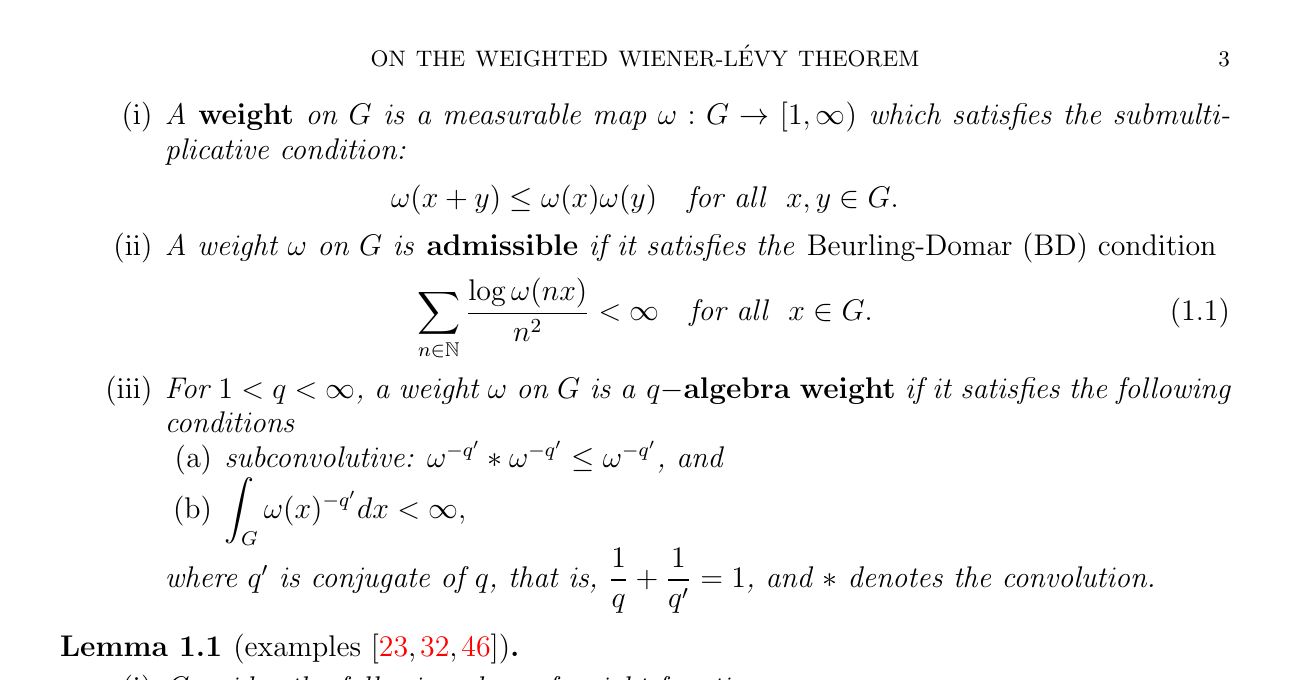
\includegraphics[width=0.96\textwidth]{figures/source_weight_definition_crop.png}
 \caption{The paper's definition on source PDF page 3.  The crop is taken
 directly from the archived v2 source PDF~\cite{BS}.}
 \label{fig:weight-definition}
\end{figure}

On $\R^d$, the paper calls a weight of \emph{regular growth} when, for
$r\ge1$,
\begin{equation}\label{eq:regular-growth}
 \omega(x/r)\le\omega(x),\qquad
 \omega(rx)\le C r^\alpha\omega(x)
\end{equation}
for some $C\ge1$ and $\alpha>0$.  Theorem 1.5 then asserts that if $\omega$
is admissible, is a $q$-algebra weight for $q>1$, and has regular growth,
every real analytic $F$ with $F(0)=0$ acts on the corresponding weighted
Fourier algebra.  Figures~\ref{fig:theorem} and~\ref{fig:remark} show the
statement and its proposed extension.

\begin{figure}[ht]
 \centering
 
\includegraphics[width=0.96\textwidth]{figures/source_theorem_crop.png}
 \caption{Regular growth and Theorem 1.5(i), source PDF page 6~\cite{BS}.}
 \label{fig:theorem}
\end{figure}

\begin{figure}[ht]
 \centering
 
\includegraphics[width=0.96\textwidth]{figures/open_problem_crop.png}
 \caption{Theorem 1.5(ii) and Remark 1.4 asking about arbitrary $\Gamma$,
 source PDF page 7~\cite{BS}.}
 \label{fig:remark}
\end{figure}
\FloatBarrier

For a weight on $\R^d$, write
\[
 L^q_\omega=\left\{g:\int_{\R^d}|g(x)|^q\omega(x)^q\,dx<\infty\right\},
 \qquad A^q_\omega=\F(L^q_\omega).
\]
Under the source hypotheses, $L^q_\omega\subset L^1$: this is immediate
for $q=1$ because $\omega\ge1$, and for $q>1$ follows from H\"older's
inequality and the second condition in~\eqref{eq:qalg-source}.  Thus the
Fourier transform is defined on $L^q_\omega$ and is injective there.

\section{Exact characterization of the obstruction}

The proof intuition is short.  Complex conjugation in physical space
reflects and conjugates the inverse Fourier datum:
\begin{equation}\label{eq:fourier-reflection}
 \overline{\widehat g}=\widehat{Jg},
 \qquad (Jg)(x)=\overline{g(-x)}.
\end{equation}
The weighted norm of $Jg$ sees $\omega(-x)$ rather than $\omega(x)$.
Consequently, conjugation preserves the Fourier algebra precisely when the
weight cannot distinguish the two half-spaces by an unbounded factor.

\begin{theorem}[Conjugation characterization]\label{thm:characterization}
Let $1\le q<\infty$ and let $\omega:\R^d\to[1,\infty)$ be a measurable
weight such that $L^q_\omega\subset L^1$.  The following are equivalent:
\begin{enumerate}[label=\textup{(\roman*)}]
 \item $f\in A^q_\omega$ implies $\overline f\in A^q_\omega$;
 \item $Jg=\overline{g(-\,\cdot)}$ maps $L^q_\omega$ into itself;
 \item there is $M<\infty$ such that
 \[
   M^{-1}\omega(x)\le\omega(-x)\le M\omega(x)
   \quad\text{for almost every }x.
 \]
\end{enumerate}
When these conditions hold, the operator norm of $J$ is
$\operatorname*{ess\,sup}_x\omega(-x)/\omega(x)$.
\end{theorem}

\begin{proof}
Identity~\eqref{eq:fourier-reflection} and Fourier injectivity on $L^1$
give the equivalence of (i) and (ii).  Indeed, if
$\overline{\widehat g}=\widehat h$ for some $h\in L^q_\omega$, then
$\widehat h=\widehat{Jg}$ and hence $h=Jg$.

If $J$ maps all of $L^q_\omega$ into itself, its graph is closed.  To see
this, suppose $g_n\to g$ and $Jg_n\to h$ in $L^q_\omega$.  Since
$\omega\ge1$, both convergences also hold in unweighted $L^q$; reflection
is an isometry there, so $Jg_n\to Jg$ and $h=Jg$.  The closed graph theorem
makes $J$ bounded.

A change of variables gives the exact identity
\begin{equation}\label{eq:Jnorm}
 \|Jg\|_{L^q_\omega}^q
 =\int_{\R^d}|g(x)|^q\omega(-x)^q\,dx.
\end{equation}
Thus $J$ is bounded if and only if
$\omega(-x)/\omega(x)$ is essentially bounded.  The necessity follows,
for example, by testing characteristic functions on finite-measure subsets
of its level sets; sufficiency follows directly from~\eqref{eq:Jnorm}.
Replacing $x$ by $-x$ supplies the reverse inequality.  Formula
\eqref{eq:Jnorm} also yields the stated norm.
\end{proof}

Since $F(z)=\overline z$ is real analytic in the paper's explicit
real-variable sense, Theorem~\ref{thm:characterization} shows that
reflection comparability is a \emph{necessary} hypothesis for the universal
real-analytic conclusion in Theorem 1.5.  We next show that none of the
other printed conditions forces it.

\section{Asymmetric weights satisfying every printed condition}

Fix real numbers $a>b\ge0$ and define
\begin{equation}\label{eq:w0}
 w_0(x)=
 \begin{cases}
  (1+x)^a,&x\ge0,\\
  (1+|x|)^b,&x<0.
 \end{cases}
\end{equation}

\begin{lemma}\label{lem:basic-weight}
The function $w_0$ is a submultiplicative weight, has regular growth, and
satisfies the Beurling--Domar condition.  Moreover,
$w_0(x)/w_0(-x)=(1+x)^{a-b}$ for $x>0$, so it is not reflection comparable.
These properties, except for the displayed normalization at zero, persist
after multiplication by any constant $L\ge1$.
\end{lemma}

\begin{proof}
For two arguments of the same sign, submultiplicativity follows from
$1+s+t\le(1+s)(1+t)$ and the appropriate exponent.  If $x\ge0>y$, then:
when $x+y\ge0$,
\[
 w_0(x+y)=(1+x-|y|)^a\le(1+x)^a\le w_0(x)w_0(y),
\]
while when $x+y<0$,
\[
 w_0(x+y)=(1+|y|-x)^b\le(1+|y|)^b\le w_0(x)w_0(y).
\]
The other mixed order is identical.

Positive dilation does not change the half-line.  Monotonicity gives
$w_0(x/r)\le w_0(x)$, and, since $a>b$,
$w_0(rx)\le r^a w_0(x)$ for $r\ge1$.  Thus~\eqref{eq:regular-growth}
holds.  Finally,
\[
 \log w_0(nx)\le a\log(1+n|x|),
\]
and the series of this expression divided by $n^2$ converges.  Multiplying
by $L\ge1$ adds $\log L$ to the Beurling--Domar estimate and gives
\[
 Lw_0(x+y)\le Lw_0(x)w_0(y)\le (Lw_0(x))(Lw_0(y)),
\]
while leaving the other arguments unchanged.
\end{proof}

For $q=1$, Lemma~\ref{lem:basic-weight} already supplies all the required
weight hypotheses; one may take $a=1$, $b=0$, and $\omega=w_0$.  For
$q>1$, the paper also requires the normalized subconvolution inequality.

\begin{lemma}[Exact $q$-algebra normalization]\label{lem:qweight}
Let $1<q<\infty$, put $r=q'$, and choose $a>b>1/r$.  Set
\begin{align*}
 C_+&=\frac{2}{br-1}+\frac{2^{ar+1}}{ar-1},\\
 C_-&=\frac{2}{ar-1}+\frac{2^{br+1}}{br-1},
 \qquad C=\max\{C_+,C_-\}.
\end{align*}
If $L\ge\max\{1,C^{1/r}\}$ and $\omega=Lw_0$, then $\omega$ is an
admissible regular-growth $q$-algebra weight in the exact sense of the
paper.
\end{lemma}

\begin{proof}
Put $v_0=w_0^{-r}$.  Since $ar>1$ and $br>1$,
\[
 \int_\R v_0(x)\,dx=\frac1{ar-1}+\frac1{br-1}<\infty.
\]
We prove $v_0*v_0\le Cv_0$.  Let $x\ge0$.  On $y<0$ we have
$v_0(x-y)\le v_0(x)$, while on $y>x$ we have $v_0(y)\le v_0(x)$.
Each tail therefore contributes at most $v_0(x)/(br-1)$.  On
$0\le y\le x$, split at $x/2$.  On the first half,
$v_0(x-y)\le2^{ar}v_0(x)$; on the second the analogous estimate holds for
$v_0(y)$.  Integrating the remaining factor over a half-line bounds the
middle contribution by
\[
 \frac{2^{ar+1}}{ar-1}v_0(x).
\]
Hence $(v_0*v_0)(x)\le C_+v_0(x)$.  For $x<0$, the same three-interval
argument with $a$ and $b$ interchanged gives
$(v_0*v_0)(x)\le C_-v_0(x)$.

Now $v=\omega^{-r}=L^{-r}v_0$, so
\[
 v*v=L^{-2r}(v_0*v_0)
 \le C L^{-2r}v_0=C L^{-r}v\le v.
\]
Together with integrability, this is exactly~\eqref{eq:qalg-source}.
Admissibility and regular growth follow from Lemma~\ref{lem:basic-weight}.
\end{proof}

\section{Counterexample for every finite \texorpdfstring{$q$}{q}}

\begin{theorem}[Full counterexample family]\label{thm:counterexample}
For every fixed $1\le q<\infty$, there exist a weight $\omega$ satisfying
all the hypotheses of Theorem 1.5 in dimension $d=1$, and an
$f\in A^q_\omega(\R)$, such that
\[
 F\circ f=\overline f\notin A^q_\omega(\R)
 \qquad\text{for }F(z)=\overline z.
\]
Consequently both parts of Theorem 1.5 are false as printed, already for
the scalar algebra $\mathcal X=\C$ and, in the multivariate part, $n=1$.
\end{theorem}

\begin{proof}
For $q=1$, take $a=1$, $b=0$ and $\omega=w_0$.  For $q>1$, choose any
$a>b>1/q'$ and take the scaled weight supplied by
Lemma~\ref{lem:qweight}.  In either case put
\[
 s=\frac{a+b}{2}+\frac1q,
 \qquad g(x)=\mathbf 1_{(-\infty,-1)}(x)|x|^{-s}.
\]
On the negative half-line,
\[
 q(s-b)=1+\frac{q(a-b)}2>1,
\]
and therefore
\[
 \int_\R |g(x)|^q\omega(x)^q\,dx<\infty.
\]
Thus $g\in L^q_\omega$.  On the other hand,
\[
 (Jg)(x)=\mathbf 1_{(1,\infty)}(x)x^{-s},
 \qquad q(s-a)=1-\frac{q(a-b)}2<1,
\]
so
\[
 \int_\R |Jg(x)|^q\omega(x)^q\,dx=\infty.
\]
Let $f=\widehat g$.  Then $f\in A^q_\omega$, whereas
$\overline f=\widehat{Jg}$ cannot belong to $A^q_\omega$ by Fourier
injectivity, exactly as in Theorem~\ref{thm:characterization}.

Finally, $F(z)=\overline z$ is a polynomial in the real variables
$z=x+iy$, namely $F(x,y)=x-iy$.  It is therefore real analytic under the
paper's Definition 1.2 and satisfies $F(0)=0$.
\end{proof}

\section{Where the source proof fails}

The source proof begins with $f=f_1+if_2$ and says that $f_1$ and $f_2$
belong to $A^q_\omega$ because they are the real and imaginary parts of
$f$; see Figure~\ref{fig:proof-flaw}.  But
\[
 \operatorname{Re}f=\frac{f+\overline f}{2},\qquad
 \operatorname{Im}f=\frac{f-\overline f}{2i},
\]
so that step requires closure under conjugation.  Theorem
\ref{thm:characterization} proves that this is equivalent to the absent
hypothesis $\omega(x)\asymp\omega(-x)$.  The counterexample makes the first
of these real/imaginary parts fail to lie in the algebra.

\begin{figure}[ht]
 \centering
 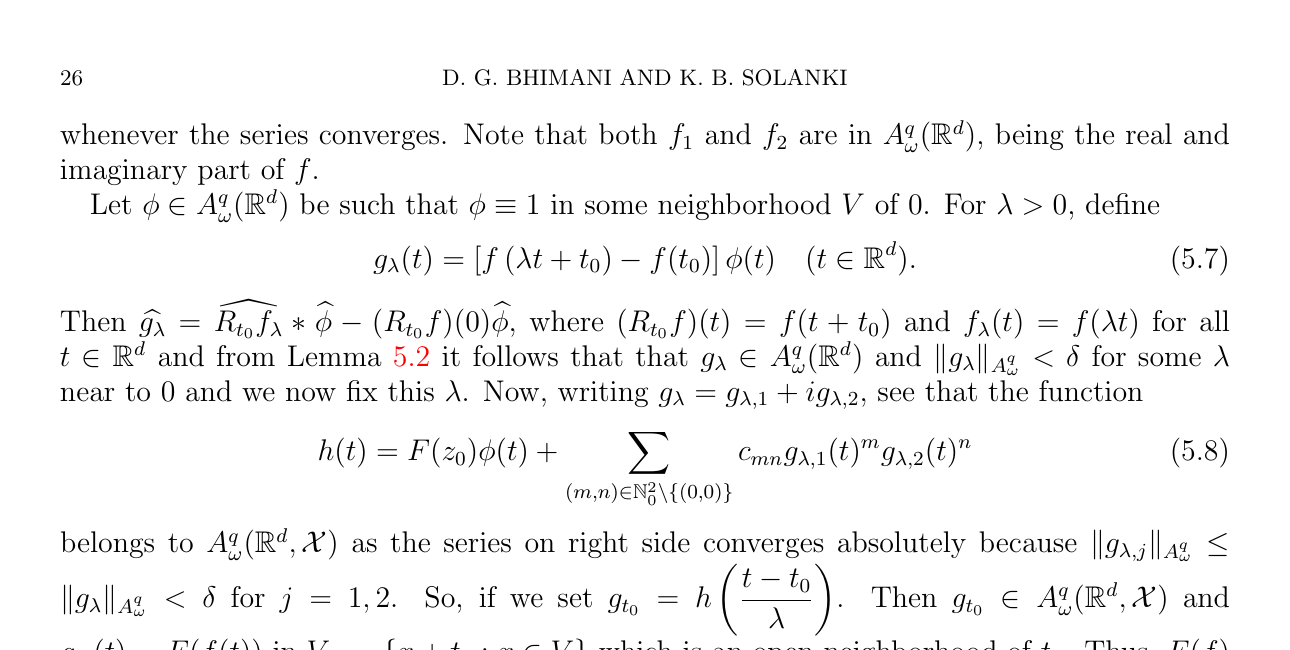
\includegraphics[width=0.96\textwidth]{figures/source_proof_flaw_crop.png}
 \caption{The unsupported real/imaginary-part step at the top of source PDF
 page 26~\cite{BS}.}
 \label{fig:proof-flaw}
\end{figure}
\FloatBarrier

The exact statement correction forced by the advertised universal
real-analytic calculus is therefore:
\begin{quote}
Add at least the hypothesis
$\omega(x)\asymp\omega(-x)$ almost everywhere.
\end{quote}
This correction is necessary and sufficient for the conjugation step.  We
do \emph{not} claim here that it is by itself sufficient to validate every
other localization and scaling step in the proof of Theorem 1.5.

Remark 1.4's proposed extension to arbitrary $\Gamma$ also cannot hold
under the same printed hypotheses: the Euclidean base statement already
fails.  This does not settle the paper's separate question of replacing
the Beurling--Domar condition by the Gelfand--Raikov--Shilov condition.

\section{Verification, interpretation, and bounded novelty}

The construction is self-contained.  Its only analytic input beyond
elementary integration is Fourier uniqueness on $L^1$ and the closed graph
theorem.  A companion script checks representative parameters for
$q=1,2,3$, evaluates the constants in Lemma~\ref{lem:qweight}, runs
deterministic random submultiplicativity tests, and numerically samples the
convolution ratio.  No numerical computation is used in the proof.

The terminology caveat is concrete.  Some authors define a ``weight'' in a
particular involutive weighted algebra to include symmetry.  Here, however,
the source gives an explicit three-part definition, and neither that
definition nor the regular-growth definition contains symmetry.  If the
authors intended a symmetric weight by convention, this packet identifies
a precise missing hypothesis and proof dependency rather than refuting the
intended symmetric statement.

A bounded search through 9 August 2026 checked the current arXiv v2 record,
the exact title and arXiv identifier together with ``counterexample'',
``correction'', and ``erratum'', and searches combining weighted Fourier or
Beurling algebras with conjugation, involution, and reflection symmetry.
Run-local indexes were also checked.  No correction or prior statement of
this exact counterexample was found.  General reflection-symmetry issues in
weighted algebras are familiar, so novelty is claimed only for the explicit
application to Theorem 1.5 and the all-$q$ construction; an exhaustive
bibliographic review was not performed.

\paragraph{Human-review recommendation.}
Check the intended convention for ``weight'' with the authors.  As a
mathematical statement under the definition printed on page 3, Theorem 1.5
is false for every finite $q$, and Theorem~\ref{thm:characterization}
pinpoints the exact missing condition for the first indispensable
real-analytic operation.

\begin{thebibliography}{9}
\bibitem{BS}
D.~G.~Bhimani and K.~B.~Solanki,
\emph{On the weighted Wiener--L\'evy theorem: analogue on Euclidean space,
strong converse on LCA group and applications to modulation spaces},
arXiv:2507.16516v2 (2025).
\end{thebibliography}

\end{document}
